\documentclass[11pt]{article}
\usepackage{geometry}
\usepackage{amsmath}
\usepackage{graphicx}
\geometry{
a4paper,
left = 22mm,
right = 22mm,
top = 15mm,
bottom = 25mm}
\title{Midterm Report: Rossmann Store Sales Prediction}
\date{\vspace{-5ex}}
\author{Hao Qian(hq43), Yuning Yang(yy693)}

\begin{document}
\maketitle
\section{Project Description}
Our project aims at modeling the sales of these Rossmann stores and predicting their 6 weeks of sales to support the stores’ daily operation. The prediction would help the specific stores to schedule their staff more efficiently. It would also help the company to find out both the most and the least profitable stores and adjust their business strategies accordingly. From the analysis, we'll also try to learn in what degree various factors contribute to the sales. 

\section{Brief Data Description}
We will use two datasets to train our models. One dataset has over 1 million records with 9 columns of store, sales, customer, competitors and promos, which are all closely related to sales results. The other dataset has one record per store, describing a store's type, recurring promos and competitors with 10 columns. In Section 4, we will describe how we deal with various fields in details.\\
We'll use the test dataset with 40k records provided by Kaggle and submit our predication results to evaluate our models. We find that some test records hold NA values on StoreOpen attribute, we fix them by checking if sales is zero.

\section{Exploratory Data Analysis}
Figure \ref{fig:promo} shows how Promo influences sales on different days of a week. We use sales data of Store No.1000 in 2015, we can learn that Promo can increase sales significantly. We can also tell from this figure that the store is closed on Sunday, it doesn't have any promos on Saturday and it influences sales differently on Monday and Friday.\\
\begin{figure}[h!]
  \centering
  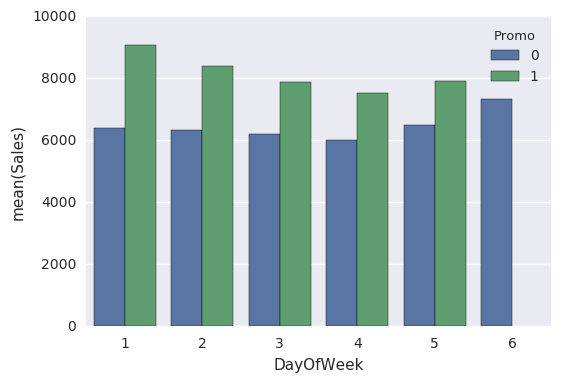
\includegraphics[scale=0.6]{promo.png}
  \caption{Mean sales of store No.1000 by DayofWeek, Promo}
  \label{fig:promo}
\end{figure}\\
Figure \ref{fig:dayofweek} shows sales distribution by day of week. We can learn from this figure that stores sell more on Monday than other weekdays. Since many stores are closed on Sunday, the open stores can have more sales than weekdays.\\
\begin{figure}[h!]
  \centering
  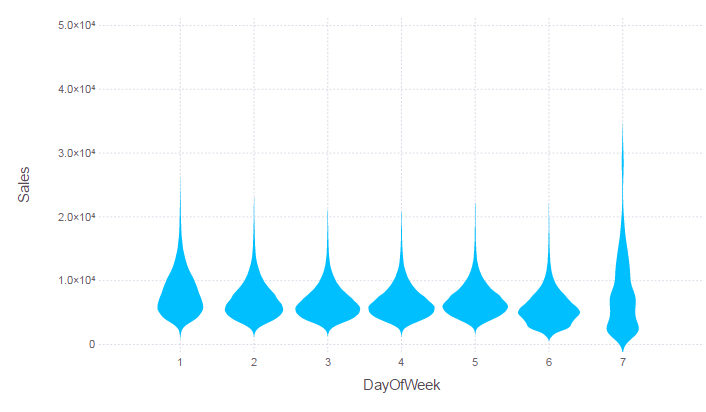
\includegraphics[scale=0.5]{DayOfWeek.PNG}
  \caption{Sales distribution on different days of a week}
  \label{fig:dayofweek}
\end{figure}\\
From Figure \ref{fig:storetype}, we can learn that different types of stores have different sales. Specifically, stores of type b often sell more goods than a,c,d. \\
\begin{figure}[h!]
  \centering
  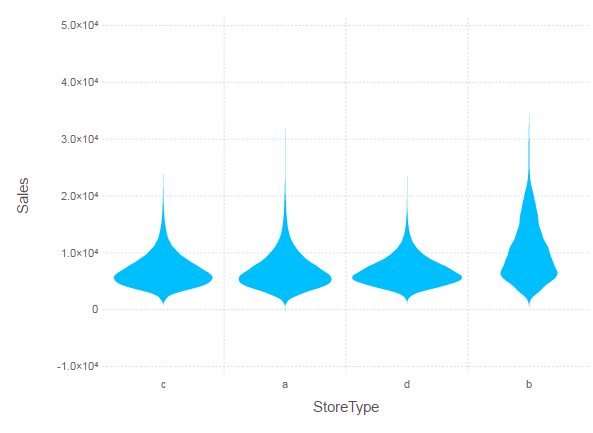
\includegraphics[scale=0.5]{StoreType.PNG}
  \caption{Sales distribution on different StoreType}
  \label{fig:storetype}
\end{figure}\\
Figure \ref{fig:competition} shows how sales changes after competitors came. We learn from store.csv that competition started from 2013.8, where we can see a dramatic decrease of sales on the figure. This figure tells us that sometimes competition can influence sales significantly.\\
\begin{figure}[h!]
  \centering
  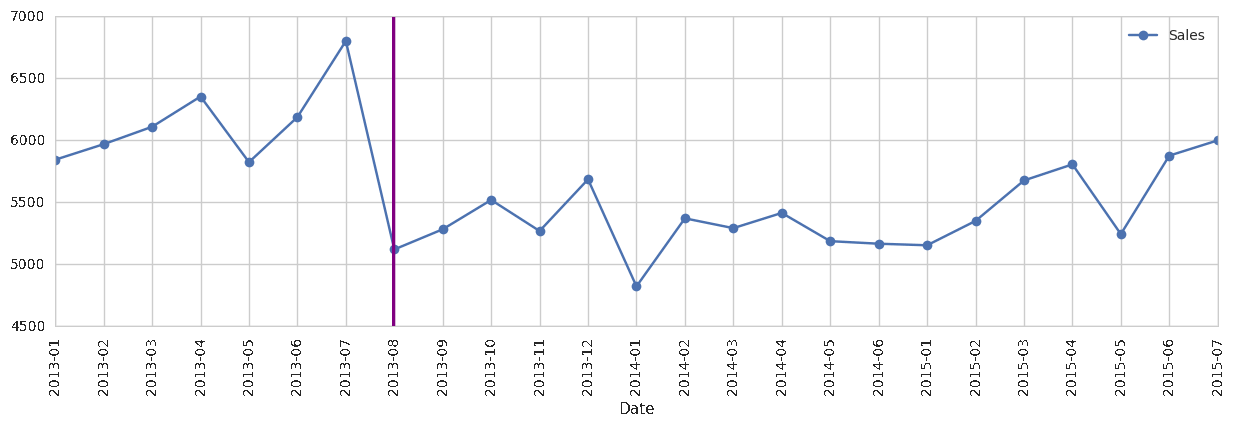
\includegraphics[scale=0.4]{competition.png}
  \caption{Sales trend of store No.191, competition since 2013.8}
  \label{fig:competition}
\end{figure}\\

\section{Feature Transformation}
As we see above, some fields are closely related the sales of stores. \\
DayOfWeek has nominal values (1,2,3,4,5,6,7). We transform categorical values to dummy variables, e.g. isMonday\{0,1\}, isSunday\{0,1\}.\\
Similarly, we transform nominal fields like StateHoliday\{a,b,c,0\}, StoreType\{a,b,c,d\}, Assortment\{a,b,c\} to dummy variables.\\
Field Promo2\{0,1\}, which indicates if a store participants in a continuing and consecutive promotion. Promo2Since\{year,week\} indicates what time the store started participating in Promo2. PromoInterval \{"Jan,Apr,Jul,Oct", "Feb,May,Aug,Nov", "Mar,Jun,Sept,Dec"\} has three values which can be treated as the type of promo2 and will be transformed to dummy variables because it's categorical. Transformed features look like (haspromo2, promo2jan, promo2feb, promo2mar, promo2since).\\
For fields (CompetitionDistance, CompetitionSince), we will check if a store has competitors at specified date, if not, we'll assign a very big value of CompetitonDistance which indicates it doesn't influence the store. In this way we can eliminate NA values of CompetitionDistance.

\section{Preliminary Predictions \& Discoveries}
To start with, we first use 4 basic features (DayOfWeek, StateHoliday, SchoolHoliday, Promotion) and 844392 examples (shops that are open) from our first dataset. Multinominal feature like DayOfWeek has been transformed as explained in previous part. 13 features are used to train our models. Constant offset is also added when doing computation. So far we have applied least sqaure and huber regression ($\sigma=1$), both with zero regularizer. Each model has different loss functions. Least sqaure minimized average error, huber regression penalized outliers less to be much robust. The performance of the models are evaluted using root mean sqaure percentage error (RMSPE).

\begin{table}[h!]
\centering
\caption{RMSPE \& some coefficients}
\label{my-label}
\begin{tabular}{|l|l|l|l|l|l|l|l|}
\hline
Model & \begin{tabular}[c]{@{}l@{}}Train\\ Error\end{tabular} & \begin{tabular}[c]{@{}l@{}}Test\\ Error\end{tabular} & IsMonday & IsSaturday & IsSunday & Promo & \begin{tabular}[c]{@{}l@{}}School\\ Holiday\end{tabular} \\ \hline
\begin{tabular}[c]{@{}l@{}}Linear\\ Regression\end{tabular} & 0.55296 & 0.45762 & 1498.44 & 497.403 & 2845.63 & 2297.75 & 229.686 \\ \hline
\begin{tabular}[c]{@{}l@{}}Huber\\ Regression\end{tabular} & 0.49203 & 0.39953 & 1314.07 & 466.426 & 1927.44 & 2188.6 & 153.836 \\ \hline
\end{tabular}
\end{table}
Preliminary results reflect parts of our discoveries in EDA. The error and some of the coefficients of the models are shown below.In all, huber regression performs better than least square. What's interesting is that train errors are larger than test errors. Both have test error around 0.4, which indicates a huge progress should be made to improve the prediction.  Specifically, the coefficients of IsMonday, IsSunday and Promotion are really large in comparison with others. These reflect the customers' preference of shopping on Monday and Sunday. When there's promotion, people are also more willing to purchase.

\section{Future Plan}
Features related to each store hasn't been used, we plan to train different coefficients for different types of stores. Besides, historical sales data is continuous time series data. We will add the new features and incorporate time series features in our future models to see if there are better predicators.\\
Most of our features are categorical or boolean variables. We will try to use some more models with regularizers that would perform better with these kinds of variables. The accuracy is not satisfying so far. Exact model parameters would also be considered carefully to get more accurate models.\\

\end{document}